\chapter{Truy vấn trên cây}

\index{tree query}
\index{truy vấn trên cây}

Chương này thảo luận về các kỹ thuật xử lý
các truy vấn trên các cây con và đường đi của một cây có gốc.
Ví dụ, các truy vấn đó là:

\begin{itemize}
\item tổ tiên thứ $k$ của một đỉnh là gì?
\item tổng các giá trị trong cây con của một đỉnh là bao nhiêu?
\item tổng các giá trị trên một đường đi giữa hai đỉnh là bao nhiêu?
\item tổ tiên chung thấp nhất của hai đỉnh là gì?
\end{itemize}

\section{Tìm tổ tiên}

\index{ancestor}
\index{tổ tiên}

\key{Tổ tiên} thứ $k$ của một đỉnh $x$ trong một cây có gốc
là đỉnh mà chúng ta sẽ đến nếu chúng ta di chuyển lên $k$
mức từ $x$.
Gọi $\texttt{ancestor}(x,k)$ là tổ tiên thứ $k$ của một đỉnh $x$
(hoặc $0$ nếu không có tổ tiên như vậy).
Ví dụ, trong cây sau,
$\texttt{ancestor}(2,1)=1$ và $\texttt{ancestor}(8,2)=4$.
\begin{center}
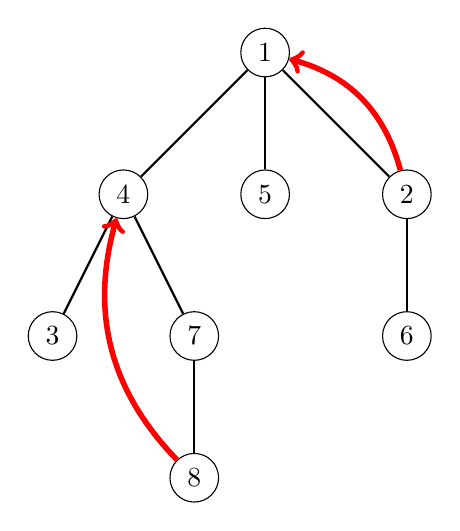
\begin{tikzpicture}[scale=0.9]
\node[draw, circle] (1) at (0,3) {$1$};
\node[draw, circle] (2) at (2,1) {$2$};
\node[draw, circle] (3) at (-2,1) {$4$};
\node[draw, circle] (4) at (0,1) {$5$};
\node[draw, circle] (5) at (2,-1) {$6$};
\node[draw, circle] (6) at (-3,-1) {$3$};
\node[draw, circle] (7) at (-1,-1) {$7$};
\node[draw, circle] (8) at (-1,-3) {$8$};
\path[draw,thick,-] (1) -- (2);
\path[draw,thick,-] (1) -- (3);
\path[draw,thick,-] (1) -- (4);
\path[draw,thick,-] (2) -- (5);
\path[draw,thick,-] (3) -- (6);
\path[draw,thick,-] (3) -- (7);
\path[draw,thick,-] (7) -- (8);

\path[draw=red,thick,->,line width=2pt] (8) edge [bend left] (3);
\path[draw=red,thick,->,line width=2pt] (2) edge [bend right] (1);
\end{tikzpicture}
\end{center}

Một cách dễ dàng để tính bất kỳ giá trị nào của $\texttt{ancestor}(x,k)$
là thực hiện một chuỗi $k$ lần di chuyển trong cây.
Tuy nhiên, độ phức tạp thời gian của phương pháp này
là $O(k)$, có thể chậm, vì một cây có $n$
đỉnh có thể có một chuỗi $n$ đỉnh.

May mắn thay, sử dụng một kỹ thuật tương tự như kỹ thuật
được sử dụng trong Chương 16.3, bất kỳ giá trị nào của $\texttt{ancestor}(x,k)$
cũng có thể được tính toán hiệu quả trong thời gian $O(\log k)$
sau khi tiền xử lý.
Ý tưởng là tiền tính toán tất cả các giá trị $\texttt{ancestor}(x,k)$
trong đó $k \le n$ là một lũy thừa của hai.
Ví dụ, các giá trị cho cây trên
như sau:

\begin{center}
\begin{tabular}{r|rrrrrrrrr}
$x$ & 1 & 2 & 3 & 4 & 5 & 6 & 7 & 8 \\
\hline
$\texttt{ancestor}(x,1)$ & 0 & 1 & 4 & 1 & 1 & 2 & 4 & 7 \\
$\texttt{ancestor}(x,2)$ & 0 & 0 & 1 & 0 & 0 & 1 & 1 & 4 \\
$\texttt{ancestor}(x,4)$ & 0 & 0 & 0 & 0 & 0 & 0 & 0 & 0 \\
$\cdots$ \\
\end{tabular}
\end{center}

Việc tiền xử lý mất thời gian $O(n \log n)$,
vì $O(\log n)$ giá trị được tính cho mỗi đỉnh.
Sau đó, bất kỳ giá trị nào của $\texttt{ancestor}(x,k)$ cũng có thể được tính
trong thời gian $O(\log k)$ bằng cách biểu diễn $k$
dưới dạng tổng các lũy thừa của hai.

\section{Cây con và đường đi}

\index{tree traversal array}
\index{mảng duyệt cây}

Một \key{mảng duyệt cây} chứa các đỉnh của một cây có gốc
theo thứ tự mà một tìm kiếm theo chiều sâu
từ đỉnh gốc duyệt qua chúng.
Ví dụ, trong cây
\begin{center}
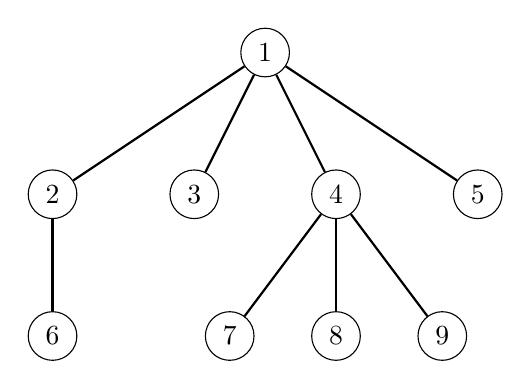
\begin{tikzpicture}[scale=0.9]
\node[draw, circle] (1) at (0,3) {$1$};
\node[draw, circle] (2) at (-3,1) {$2$};
\node[draw, circle] (3) at (-1,1) {$3$};
\node[draw, circle] (4) at (1,1) {$4$};
\node[draw, circle] (5) at (3,1) {$5$};
\node[draw, circle] (6) at (-3,-1) {$6$};
\node[draw, circle] (7) at (-0.5,-1) {$7$};
\node[draw, circle] (8) at (1,-1) {$8$};
\node[draw, circle] (9) at (2.5,-1) {$9$};

\path[draw,thick,-] (1) -- (2);
\path[draw,thick,-] (1) -- (3);
\path[draw,thick,-] (1) -- (4);
\path[draw,thick,-] (1) -- (5);
\path[draw,thick,-] (2) -- (6);
\path[draw,thick,-] (4) -- (7);
\path[draw,thick,-] (4) -- (8);
\path[draw,thick,-] (4) -- (9);
\end{tikzpicture}
\end{center}
một tìm kiếm theo chiều sâu diễn ra như sau:
\begin{center}
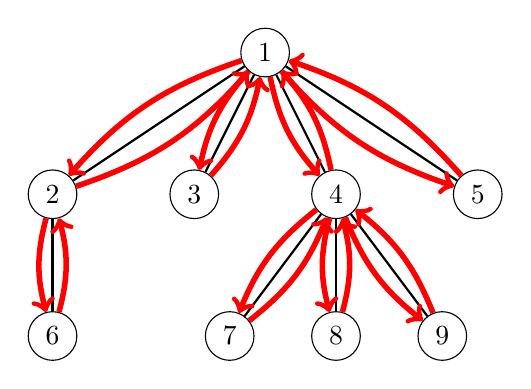
\begin{tikzpicture}[scale=0.9]
\node[draw, circle] (1) at (0,3) {$1$};
\node[draw, circle] (2) at (-3,1) {$2$};
\node[draw, circle] (3) at (-1,1) {$3$};
\node[draw, circle] (4) at (1,1) {$4$};
\node[draw, circle] (5) at (3,1) {$5$};
\node[draw, circle] (6) at (-3,-1) {$6$};
\node[draw, circle] (7) at (-0.5,-1) {$7$};
\node[draw, circle] (8) at (1,-1) {$8$};
\node[draw, circle] (9) at (2.5,-1) {$9$};

\path[draw,thick,-] (1) -- (2);
\path[draw,thick,-] (1) -- (3);
\path[draw,thick,-] (1) -- (4);
\path[draw,thick,-] (1) -- (5);
\path[draw,thick,-] (2) -- (6);
\path[draw,thick,-] (4) -- (7);
\path[draw,thick,-] (4) -- (8);
\path[draw,thick,-] (4) -- (9);


\path[draw=red,thick,->,line width=2pt] (1) edge [bend right=15] (2);
\path[draw=red,thick,->,line width=2pt] (2) edge [bend right=15] (6);
\path[draw=red,thick,->,line width=2pt] (6) edge [bend right=15] (2);
\path[draw=red,thick,->,line width=2pt] (2) edge [bend right=15] (1);
\path[draw=red,thick,->,line width=2pt] (1) edge [bend right=15] (3);
\path[draw=red,thick,->,line width=2pt] (3) edge [bend right=15] (1);
\path[draw=red,thick,->,line width=2pt] (1) edge [bend right=15] (4);
\path[draw=red,thick,->,line width=2pt] (4) edge [bend right=15] (7);
\path[draw=red,thick,->,line width=2pt] (7) edge [bend right=15] (4);
\path[draw=red,thick,->,line width=2pt] (4) edge [bend right=15] (8);
\path[draw=red,thick,->,line width=2pt] (8) edge [bend right=15] (4);
\path[draw=red,thick,->,line width=2pt] (4) edge [bend right=15] (9);
\path[draw=red,thick,->,line width=2pt] (9) edge [bend right=15] (4);
\path[draw=red,thick,->,line width=2pt] (4) edge [bend right=15] (1);
\path[draw=red,thick,->,line width=2pt] (1) edge [bend right=15] (5);
\path[draw=red,thick,->,line width=2pt] (5) edge [bend right=15] (1);

\end{tikzpicture}
\end{center}
Do đó, mảng duyệt cây tương ứng như sau:
\begin{center}
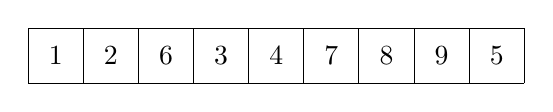
\begin{tikzpicture}[scale=0.7]
\draw (0,0) grid (9,1);

\node at (0.5,0.5) {$1$};
\node at (1.5,0.5) {$2$};
\node at (2.5,0.5) {$6$};
\node at (3.5,0.5) {$3$};
\node at (4.5,0.5) {$4$};
\node at (5.5,0.5) {$7$};
\node at (6.5,0.5) {$8$};
\node at (7.5,0.5) {$9$};
\node at (8.5,0.5) {$5$};
% 
% \footnotesize
% \node at (0.5,1.4) {$1$};
% \node at (1.5,1.4) {$2$};
% \node at (2.5,1.4) {$3$};
% \node at (3.5,1.4) {$4$};
% \node at (4.5,1.4) {$5$};
% \node at (5.5,1.4) {$6$};
% \node at (6.5,1.4) {$7$};
% \node at (7.5,1.4) {$8$};
% \node at (8.5,1.4) {$9$};
\end{tikzpicture}
\end{center}

\subsubsection{Truy vấn cây con}

Mỗi cây con của một cây tương ứng với một mảng con
của mảng duyệt cây sao cho
phần tử đầu tiên của mảng con là đỉnh gốc.
Ví dụ, mảng con sau đây chứa các
đỉnh của cây con của đỉnh $4$:
\begin{center}
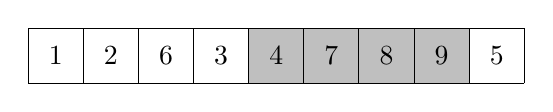
\begin{tikzpicture}[scale=0.7]
\fill[color=lightgray] (4,0) rectangle (8,1);
\draw (0,0) grid (9,1);

\node at (0.5,0.5) {$1$};
\node at (1.5,0.5) {$2$};
\node at (2.5,0.5) {$6$};
\node at (3.5,0.5) {$3$};
\node at (4.5,0.5) {$4$};
\node at (5.5,0.5) {$7$};
\node at (6.5,0.5) {$8$};
\node at (7.5,0.5) {$9$};
\node at (8.5,0.5) {$5$};
% 
% \footnotesize
% \node at (0.5,1.4) {$1$};
% \node at (1.5,1.4) {$2$};
% \node at (2.5,1.4) {$3$};
% \node at (3.5,1.4) {$4$};
% \node at (4.5,1.4) {$5$};
% \node at (5.5,1.4) {$6$};
% \node at (6.5,1.4) {$7$};
% \node at (7.5,1.4) {$8$};
% \node at (8.5,1.4) {$9$};
\end{tikzpicture}
\end{center}
Sử dụng thực tế này, chúng ta có thể xử lý hiệu quả các truy vấn
liên quan đến các cây con của một cây.
Ví dụ, hãy xem xét một bài toán trong đó mỗi đỉnh
được gán một giá trị, và nhiệm vụ của chúng ta là hỗ trợ
các truy vấn sau:
\begin{itemize}
\item cập nhật giá trị của một đỉnh
\item tính tổng các giá trị trong cây con của một đỉnh
\end{itemize}

Hãy xem xét cây sau đây trong đó các số màu xanh
là giá trị của các đỉnh.
Ví dụ, tổng của cây con của đỉnh $4$
là $3+4+3+1=11$.

\begin{center}
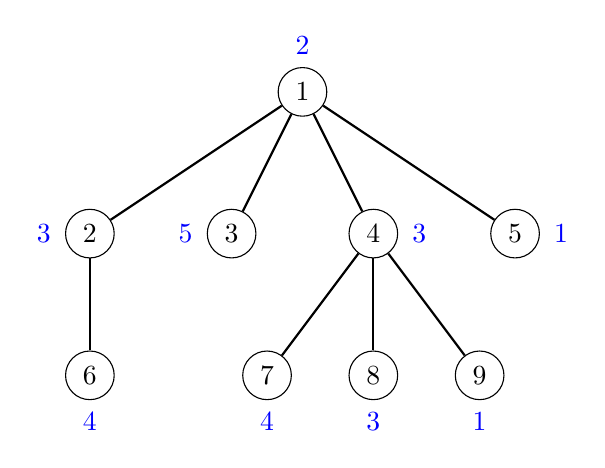
\begin{tikzpicture}[scale=0.9]
\node[draw, circle] (1) at (0,3) {$1$};
\node[draw, circle] (2) at (-3,1) {$2$};
\node[draw, circle] (3) at (-1,1) {$3$};
\node[draw, circle] (4) at (1,1) {$4$};
\node[draw, circle] (5) at (3,1) {$5$};
\node[draw, circle] (6) at (-3,-1) {$6$};
\node[draw, circle] (7) at (-0.5,-1) {$7$};
\node[draw, circle] (8) at (1,-1) {$8$};
\node[draw, circle] (9) at (2.5,-1) {$9$};

\path[draw,thick,-] (1) -- (2);
\path[draw,thick,-] (1) -- (3);
\path[draw,thick,-] (1) -- (4);
\path[draw,thick,-] (1) -- (5);
\path[draw,thick,-] (2) -- (6);
\path[draw,thick,-] (4) -- (7);
\path[draw,thick,-] (4) -- (8);
\path[draw,thick,-] (4) -- (9);

\node[color=blue] at (0,3+0.65) {2};
\node[color=blue] at (-3-0.65,1) {3};
\node[color=blue] at (-1-0.65,1) {5};
\node[color=blue] at (1+0.65,1) {3};
\node[color=blue] at (3+0.65,1) {1};
\node[color=blue] at (-3,-1-0.65) {4};
\node[color=blue] at (-0.5,-1-0.65) {4};
\node[color=blue] at (1,-1-0.65) {3};
\node[color=blue] at (2.5,-1-0.65) {1};
\end{tikzpicture}
\end{center}

Ý tưởng là xây dựng một mảng duyệt cây chứa
ba giá trị cho mỗi đỉnh: định danh của đỉnh,
kích thước của cây con, và giá trị của đỉnh.
Ví dụ, mảng cho cây trên như sau:

\begin{center}
\begin{tikzpicture}[scale=0.7]
\draw (0,1) grid (9,-2);

\node[left] at (-1,0.5) {định danh đỉnh};
\node[left] at (-1,-0.5) {kích thước cây con};
\node[left] at (-1,-1.5) {giá trị đỉnh};

\node at (0.5,0.5) {$1$};
\node at (1.5,0.5) {$2$};
\node at (2.5,0.5) {$6$};
\node at (3.5,0.5) {$3$};
\node at (4.5,0.5) {$4$};
\node at (5.5,0.5) {$7$};
\node at (6.5,0.5) {$8$};
\node at (7.5,0.5) {$9$};
\node at (8.5,0.5) {$5$};

\node at (0.5,-0.5) {$9$};
\node at (1.5,-0.5) {$2$};
\node at (2.5,-0.5) {$1$};
\node at (3.5,-0.5) {$1$};
\node at (4.5,-0.5) {$4$};
\node at (5.5,-0.5) {$1$};
\node at (6.5,-0.5) {$1$};
\node at (7.5,-0.5) {$1$};
\node at (8.5,-0.5) {$1$};

\node at (0.5,-1.5) {$2$};
\node at (1.5,-1.5) {$3$};
\node at (2.5,-1.5) {$4$};
\node at (3.5,-1.5) {$5$};
\node at (4.5,-1.5) {$3$};
\node at (5.5,-1.5) {$4$};
\node at (6.5,-1.5) {$3$};
\node at (7.5,-1.5) {$1$};
\node at (8.5,-1.5) {$1$};
% 
% \footnotesize
% \node at (0.5,1.4) {$1$};
% \node at (1.5,1.4) {$2$};
% \node at (2.5,1.4) {$3$};
% \node at (3.5,1.4) {$4$};
% \node at (4.5,1.4) {$5$};
% \node at (5.5,1.4) {$6$};
% \node at (6.5,1.4) {$7$};
% \node at (7.5,1.4) {$8$};
% \node at (8.5,1.4) {$9$};
\end{tikzpicture}
\end{center}

Sử dụng mảng này, chúng ta có thể tính tổng các giá trị
trong bất kỳ cây con nào bằng cách trước tiên tìm ra kích thước của cây con
và sau đó là giá trị của các đỉnh tương ứng.
Ví dụ, các giá trị trong cây con của đỉnh $4$
có thể được tìm thấy như sau:

\begin{center}
\begin{tikzpicture}[scale=0.7]
\fill[color=lightgray] (4,1) rectangle (5,0);
\fill[color=lightgray] (4,0) rectangle (5,-1);
\fill[color=lightgray] (4,-1) rectangle (8,-2);
\draw (0,1) grid (9,-2);

\node[left] at (-1,0.5) {định danh đỉnh};
\node[left] at (-1,-0.5) {kích thước cây con};
\node[left] at (-1,-1.5) {giá trị đỉnh};

\node at (0.5,0.5) {$1$};
\node at (1.5,0.5) {$2$};
\node at (2.5,0.5) {$6$};
\node at (3.5,0.5) {$3$};
\node at (4.5,0.5) {$4$};
\node at (5.5,0.5) {$7$};
\node at (6.5,0.5) {$8$};
\node at (7.5,0.5) {$9$};
\node at (8.5,0.5) {$5$};

\node at (0.5,-0.5) {$9$};
\node at (1.5,-0.5) {$2$};
\node at (2.5,-0.5) {$1$};
\node at (3.5,-0.5) {$1$};
\node at (4.5,-0.5) {$4$};
\node at (5.5,-0.5) {$1$};
\node at (6.5,-0.5) {$1$};
\node at (7.5,-0.5) {$1$};
\node at (8.5,-0.5) {$1$};

\node at (0.5,-1.5) {$2$};
\node at (1.5,-1.5) {$3$};
\node at (2.5,-1.5) {$4$};
\node at (3.5,-1.5) {$5$};
\node at (4.5,-1.5) {$3$};
\node at (5.5,-1.5) {$4$};
\node at (6.5,-1.5) {$3$};
\node at (7.5,-1.5) {$1$};
\node at (8.5,-1.5) {$1$};
% 
% \footnotesize
% \node at (0.5,1.4) {$1$};
% \node at (1.5,1.4) {$2$};
% \node at (2.5,1.4) {$3$};
% \node at (3.5,1.4) {$4$};
% \node at (4.5,1.4) {$5$};
% \node at (5.5,1.4) {$6$};
% \node at (6.5,1.4) {$7$};
% \node at (7.5,1.4) {$8$};
% \node at (8.5,1.4) {$9$};
\end{tikzpicture}
\end{center}

Để trả lời các truy vấn một cách hiệu quả,
chỉ cần lưu trữ các giá trị của các
đỉnh trong một cây chỉ số nhị phân hoặc cây phân đoạn.
Sau đó, chúng ta có thể vừa cập nhật một giá trị
vừa tính tổng các giá trị trong thời gian $O(\log n)$.

\subsubsection{Truy vấn đường đi}

Sử dụng một mảng duyệt cây, chúng ta cũng có thể tính toán hiệu quả
tổng các giá trị trên
các đường đi từ đỉnh gốc đến bất kỳ
đỉnh nào của cây.
Hãy xem xét một bài toán trong đó nhiệm vụ của chúng ta
là hỗ trợ các truy vấn sau:
\begin{itemize}
\item thay đổi giá trị của một đỉnh
\item tính tổng các giá trị trên một đường đi từ
gốc đến một đỉnh
\end{itemize}

Ví dụ, trong cây sau,
tổng các giá trị từ đỉnh gốc đến đỉnh 7 là
$4+5+5=14$:

\begin{center}
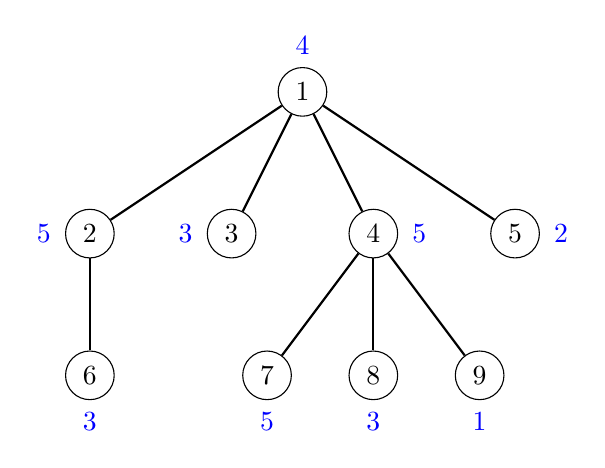
\begin{tikzpicture}[scale=0.9]
\node[draw, circle] (1) at (0,3) {$1$};
\node[draw, circle] (2) at (-3,1) {$2$};
\node[draw, circle] (3) at (-1,1) {$3$};
\node[draw, circle] (4) at (1,1) {$4$};
\node[draw, circle] (5) at (3,1) {$5$};
\node[draw, circle] (6) at (-3,-1) {$6$};
\node[draw, circle] (7) at (-0.5,-1) {$7$};
\node[draw, circle] (8) at (1,-1) {$8$};
\node[draw, circle] (9) at (2.5,-1) {$9$};

\path[draw,thick,-] (1) -- (2);
\path[draw,thick,-] (1) -- (3);
\path[draw,thick,-] (1) -- (4);
\path[draw,thick,-] (1) -- (5);
\path[draw,thick,-] (2) -- (6);
\path[draw,thick,-] (4) -- (7);
\path[draw,thick,-] (4) -- (8);
\path[draw,thick,-] (4) -- (9);

\node[color=blue] at (0,3+0.65) {4};
\node[color=blue] at (-3-0.65,1) {5};
\node[color=blue] at (-1-0.65,1) {3};
\node[color=blue] at (1+0.65,1) {5};
\node[color=blue] at (3+0.65,1) {2};
\node[color=blue] at (-3,-1-0.65) {3};
\node[color=blue] at (-0.5,-1-0.65) {5};
\node[color=blue] at (1,-1-0.65) {3};
\node[color=blue] at (2.5,-1-0.65) {1};
\end{tikzpicture}
\end{center}

Chúng ta có thể giải quyết bài toán này như trước,
nhưng bây giờ mỗi giá trị trong hàng cuối cùng của mảng là tổng các giá trị
trên một đường đi từ gốc đến đỉnh.
Ví dụ, mảng sau đây tương ứng với cây trên:
\begin{center}
\begin{tikzpicture}[scale=0.7]
\draw (0,1) grid (9,-2);

\node[left] at (-1,0.5) {định danh đỉnh};
\node[left] at (-1,-0.5) {kích thước cây con};
\node[left] at (-1,-1.5) {tổng đường đi};

\node at (0.5,0.5) {$1$};
\node at (1.5,0.5) {$2$};
\node at (2.5,0.5) {$6$};
\node at (3.5,0.5) {$3$};
\node at (4.5,0.5) {$4$};
\node at (5.5,0.5) {$7$};
\node at (6.5,0.5) {$8$};
\node at (7.5,0.5) {$9$};
\node at (8.5,0.5) {$5$};

\node at (0.5,-0.5) {$9$};
\node at (1.5,-0.5) {$2$};
\node at (2.5,-0.5) {$1$};
\node at (3.5,-0.5) {$1$};
\node at (4.5,-0.5) {$4$};
\node at (5.5,-0.5) {$1$};
\node at (6.5,-0.5) {$1$};
\node at (7.5,-0.5) {$1$};
\node at (8.5,-0.5) {$1$};

\node at (0.5,-1.5) {$2$};
\node at (1.5,-1.5) {$3$};
\node at (2.5,-1.5) {$4$};
\node at (3.5,-1.5) {$5$};
\node at (4.5,-1.5) {$3$};
\node at (5.5,-1.5) {$4$};
\node at (6.5,-1.5) {$3$};
\node at (7.5,-1.5) {$1$};
\node at (8.5,-1.5) {$1$};
% 
% \footnotesize
% \node at (0.5,1.4) {$1$};
% \node at (1.5,1.4) {$2$};
% \node at (2.5,1.4) {$3$};
% \node at (3.5,1.4) {$4$};
% \node at (4.5,1.4) {$5$};
% \node at (5.5,1.4) {$6$};
% \node at (6.5,1.4) {$7$};
% \node at (7.5,1.4) {$8$};
% \node at (8.5,1.4) {$9$};
\end{tikzpicture}
\end{center}

Khi giá trị của một đỉnh tăng thêm $x$,
tổng của tất cả các đỉnh trong cây con của nó tăng thêm $x$.
Ví dụ, nếu giá trị của đỉnh 4 tăng thêm 1,
mảng thay đổi như sau:

\begin{center}
\begin{tikzpicture}[scale=0.7]
\fill[color=lightgray] (4,-1) rectangle (8,-2);
\draw (0,1) grid (9,-2);

\node[left] at (-1,0.5) {định danh đỉnh};
\node[left] at (-1,-0.5) {kích thước cây con};
\node[left] at (-1,-1.5) {tổng đường đi};

\node at (0.5,0.5) {$1$};
\node at (1.5,0.5) {$2$};
\node at (2.5,0.5) {$6$};
\node at (3.5,0.5) {$3$};
\node at (4.5,0.5) {$4$};
\node at (5.5,0.5) {$7$};
\node at (6.5,0.5) {$8$};
\node at (7.5,0.5) {$9$};
\node at (8.5,0.5) {$5$};

\node at (0.5,-0.5) {$9$};
\node at (1.5,-0.5) {$2$};
\node at (2.5,-0.5) {$1$};
\node at (3.5,-0.5) {$1$};
\node at (4.5,-0.5) {$4$};
\node at (5.5,-0.5) {$1$};
\node at (6.5,-0.5) {$1$};
\node at (7.5,-0.5) {$1$};
\node at (8.5,-0.5) {$1$};

\node at (0.5,-1.5) {$2$};
\node at (1.5,-1.5) {$3$};
\node at (2.5,-1.5) {$4$};
\node at (3.5,-1.5) {$5$};
\node at (4.5,-1.5) {$3$};
\node at (5.5,-1.5) {$4$};
\node at (6.5,-1.5) {$3$};
\node at (7.5,-1.5) {$1$};
\node at (8.5,-1.5) {$1$};
% 
% \footnotesize
% \node at (0.5,1.4) {$1$};
% \node at (1.5,1.4) {$2$};
% \node at (2.5,1.4) {$3$};
% \node at (3.5,1.4) {$4$};
% \node at (4.5,1.4) {$5$};
% \node at (5.5,1.4) {$6$};
% \node at (6.5,1.4) {$7$};
% \node at (7.5,1.4) {$8$};
% \node at (8.5,1.4) {$9$};
\end{tikzpicture}
\end{center}

Một lần nữa, chúng ta có thể sử dụng một cây chỉ số nhị phân hoặc cây phân đoạn
để thực hiện các thao tác này một cách hiệu quả.
Một truy vấn tổng đường đi có thể được trả lời bằng một truy vấn điểm,
và một cập nhật giá trị tương ứng với một truy vấn phạm vi
cộng một giá trị vào một phạm vi.
Cả hai thao tác đều có thể được thực hiện trong thời gian $O(\log n)$.

\section{Tổ tiên chung thấp nhất}

\index{lowest common ancestor}
\index{tổ tiên chung thấp nhất}

Tổ tiên chung thấp nhất
của hai đỉnh của một cây có gốc là đỉnh thấp nhất
mà cây con của nó chứa cả hai đỉnh.
Một bài toán điển hình là xử lý hiệu quả
các truy vấn yêu cầu tìm tổ tiên chung thấp nhất
của hai đỉnh.

Ví dụ, trong cây sau,
tổ tiên chung thấp nhất của các đỉnh 5 và 8
là đỉnh 2:
\begin{center}
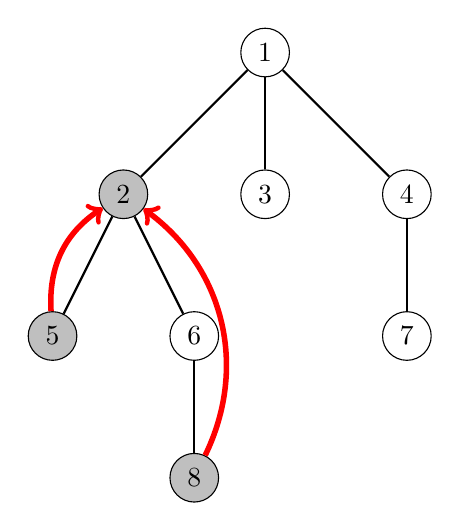
\begin{tikzpicture}[scale=0.9]
\node[draw, circle] (1) at (0,3) {$1$};
\node[draw, circle] (2) at (2,1) {$4$};
\node[draw, circle, fill=lightgray] (3) at (-2,1) {$2$};
\node[draw, circle] (4) at (0,1) {$3$};
\node[draw, circle] (5) at (2,-1) {$7$};
\node[draw, circle, fill=lightgray] (6) at (-3,-1) {$5$};
\node[draw, circle] (7) at (-1,-1) {$6$};
\node[draw, circle, fill=lightgray] (8) at (-1,-3) {$8$};
\path[draw,thick,-] (1) -- (2);
\path[draw,thick,-] (1) -- (3);
\path[draw,thick,-] (1) -- (4);
\path[draw,thick,-] (2) -- (5);
\path[draw,thick,-] (3) -- (6);
\path[draw,thick,-] (3) -- (7);
\path[draw,thick,-] (7) -- (8);

\path[draw=red,thick,->,line width=2pt] (6) edge [bend left] (3);
\path[draw=red,thick,->,line width=2pt] (8) edge [bend right=40] (3);
\end{tikzpicture}
\end{center}

Tiếp theo, chúng ta sẽ thảo luận về hai kỹ thuật hiệu quả để
tìm tổ tiên chung thấp nhất của hai đỉnh.

\subsubsection{Phương pháp 1}

Một cách để giải quyết vấn đề là sử dụng thực tế
rằng chúng ta có thể tìm thấy tổ tiên thứ $k$
của bất kỳ đỉnh nào trong cây một cách hiệu quả.
Sử dụng điều này, chúng ta có thể chia vấn đề
tìm tổ tiên chung thấp nhất thành hai phần.

Chúng ta sử dụng hai con trỏ ban đầu trỏ đến
hai đỉnh mà tổ tiên chung thấp nhất của chúng ta nên tìm.
Đầu tiên, chúng ta di chuyển một trong các con trỏ lên trên
để cả hai con trỏ đều trỏ đến các đỉnh ở cùng một cấp độ.

Trong kịch bản ví dụ, chúng ta di chuyển con trỏ thứ hai lên một
cấp độ để nó trỏ đến đỉnh 6
nằm ở cùng cấp độ với đỉnh 5:

\begin{center}
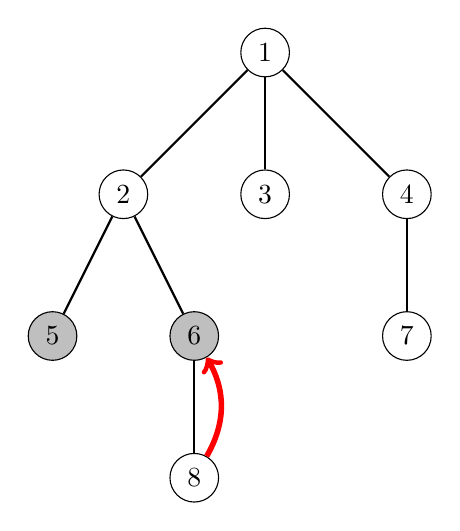
\begin{tikzpicture}[scale=0.9]
\node[draw, circle] (1) at (0,3) {$1$};
\node[draw, circle] (2) at (2,1) {$4$};
\node[draw, circle] (3) at (-2,1) {$2$};
\node[draw, circle] (4) at (0,1) {$3$};
\node[draw, circle] (5) at (2,-1) {$7$};
\node[draw, circle,fill=lightgray] (6) at (-3,-1) {$5$};
\node[draw, circle,fill=lightgray] (7) at (-1,-1) {$6$};
\node[draw, circle] (8) at (-1,-3) {$8$};
\path[draw,thick,-] (1) -- (2);
\path[draw,thick,-] (1) -- (3);
\path[draw,thick,-] (1) -- (4);
\path[draw,thick,-] (2) -- (5);
\path[draw,thick,-] (3) -- (6);
\path[draw,thick,-] (3) -- (7);
\path[draw,thick,-] (7) -- (8);

\path[draw=red,thick,->,line width=2pt] (8) edge [bend right] (7);
\end{tikzpicture}
\end{center}

Sau đó, chúng ta xác định số bước tối thiểu cần thiết
để di chuyển cả hai con trỏ lên trên để
chúng sẽ trỏ đến cùng một đỉnh.
Đỉnh mà các con trỏ trỏ đến sau đó
chính là tổ tiên chung thấp nhất.

Trong kịch bản ví dụ, chỉ cần di chuyển cả hai con trỏ
một bước lên trên đến đỉnh 2,
đó là tổ tiên chung thấp nhất:

\begin{center}
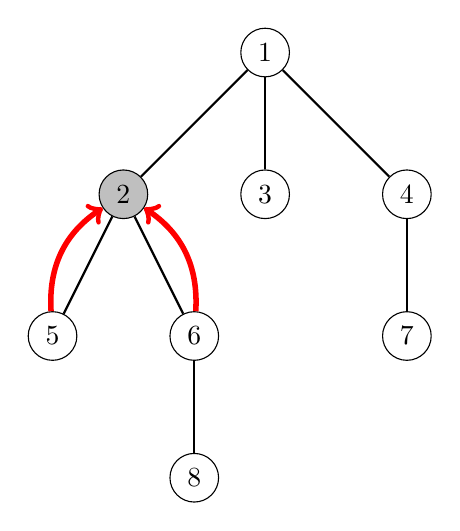
\begin{tikzpicture}[scale=0.9]
\node[draw, circle] (1) at (0,3) {$1$};
\node[draw, circle] (2) at (2,1) {$4$};
\node[draw, circle,fill=lightgray] (3) at (-2,1) {$2$};
\node[draw, circle] (4) at (0,1) {$3$};
\node[draw, circle] (5) at (2,-1) {$7$};
\node[draw, circle] (6) at (-3,-1) {$5$};
\node[draw, circle] (7) at (-1,-1) {$6$};
\node[draw, circle] (8) at (-1,-3) {$8$};
\path[draw,thick,-] (1) -- (2);
\path[draw,thick,-] (1) -- (3);
\path[draw,thick,-] (1) -- (4);
\path[draw,thick,-] (2) -- (5);
\path[draw,thick,-] (3) -- (6);
\path[draw,thick,-] (3) -- (7);
\path[draw,thick,-] (7) -- (8);

\path[draw=red,thick,->,line width=2pt] (6) edge [bend left] (3);
\path[draw=red,thick,->,line width=2pt] (7) edge [bend right] (3);
\end{tikzpicture}
\end{center}

Vì cả hai phần của thuật toán có thể được thực hiện trong
thời gian $O(\log n)$ bằng cách sử dụng thông tin đã được tính trước,
chúng ta có thể tìm tổ tiên chung thấp nhất của bất kỳ hai
đỉnh nào trong thời gian $O(\log n)$.

\subsubsection{Phương pháp 2}

\index{Euler tour technique}
\index{kỹ thuật tour Euler}

Một cách khác để giải quyết vấn đề dựa trên
một mảng duyệt cây\footnote{Thuật toán tổ tiên chung thấp nhất này đã được trình bày trong \cite{ben00}.
Kỹ thuật này đôi khi được gọi là \key{kỹ thuật tour Euler} \cite{tar84}.}.
Một lần nữa, ý tưởng là duyệt qua các đỉnh
bằng cách sử dụng một tìm kiếm theo chiều sâu:

\begin{center}
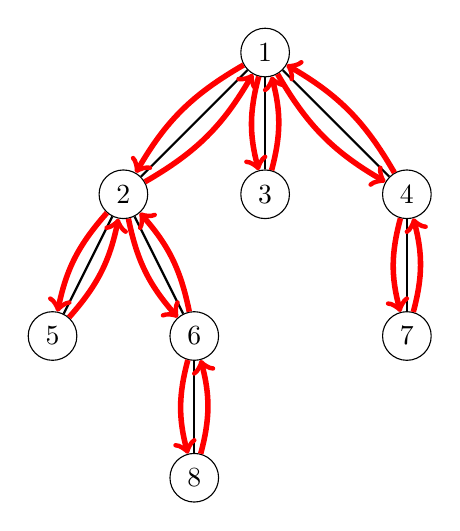
\begin{tikzpicture}[scale=0.9]
\node[draw, circle] (1) at (0,3) {$1$};
\node[draw, circle] (2) at (2,1) {$4$};
\node[draw, circle] (3) at (-2,1) {$2$};
\node[draw, circle] (4) at (0,1) {$3$};
\node[draw, circle] (5) at (2,-1) {$7$};
\node[draw, circle] (6) at (-3,-1) {$5$};
\node[draw, circle] (7) at (-1,-1) {$6$};
\node[draw, circle] (8) at (-1,-3) {$8$};
\path[draw,thick,-] (1) -- (2);
\path[draw,thick,-] (1) -- (3);
\path[draw,thick,-] (1) -- (4);
\path[draw,thick,-] (2) -- (5);
\path[draw,thick,-] (3) -- (6);
\path[draw,thick,-] (3) -- (7);
\path[draw,thick,-] (7) -- (8);

\path[draw=red,thick,->,line width=2pt] (1) edge [bend right=15] (3);
\path[draw=red,thick,->,line width=2pt] (3) edge [bend right=15] (6);
\path[draw=red,thick,->,line width=2pt] (6) edge [bend right=15] (3);
\path[draw=red,thick,->,line width=2pt] (3) edge [bend right=15] (7);
\path[draw=red,thick,->,line width=2pt] (7) edge [bend right=15] (8);
\path[draw=red,thick,->,line width=2pt] (8) edge [bend right=15] (7);
\path[draw=red,thick,->,line width=2pt] (7) edge [bend right=15] (3);
\path[draw=red,thick,->,line width=2pt] (3) edge [bend right=15] (1);
\path[draw=red,thick,->,line width=2pt] (1) edge [bend right=15] (4);
\path[draw=red,thick,->,line width=2pt] (4) edge [bend right=15] (1);
\path[draw=red,thick,->,line width=2pt] (1) edge [bend right=15] (2);
\path[draw=red,thick,->,line width=2pt] (2) edge [bend right=15] (5);
\path[draw=red,thick,->,line width=2pt] (5) edge [bend right=15] (2);
\path[draw=red,thick,->,line width=2pt] (2) edge [bend right=15] (1);
\end{tikzpicture}
\end{center}

Tuy nhiên, chúng ta sử dụng một mảng duyệt cây khác với trước:
chúng ta thêm mỗi đỉnh vào mảng \emph{luôn luôn}
khi tìm kiếm theo chiều sâu đi qua đỉnh đó,
và không chỉ trong lần truy cập đầu tiên.
Do đó, một đỉnh có $k$ con sẽ xuất hiện $k+1$ lần
trong mảng và tổng cộng có $2n-1$
đỉnh trong mảng.

Chúng ta lưu trữ hai giá trị trong mảng:
định danh của đỉnh và độ sâu của đỉnh trong cây.
Mảng sau đây tương ứng với cây trên:

\begin{center}
\begin{tikzpicture}[scale=0.7]

\node[left] at (-1,1.5) {định danh đỉnh};
\node[left] at (-1,0.5) {độ sâu};

\draw (0,1) grid (15,2);
\node at (0.5,1.5) {$1$};
\node at (1.5,1.5) {$2$};
\node at (2.5,1.5) {$5$};
\node at (3.5,1.5) {$2$};
\node at (4.5,1.5) {$6$};
\node at (5.5,1.5) {$8$};
\node at (6.5,1.5) {$6$};
\node at (7.5,1.5) {$2$};
\node at (8.5,1.5) {$1$};
\node at (9.5,1.5) {$3$};
\node at (10.5,1.5) {$1$};
\node at (11.5,1.5) {$4$};
\node at (12.5,1.5) {$7$};
\node at (13.5,1.5) {$4$};
\node at (14.5,1.5) {$1$};

\draw (0,0) grid (15,1);
\node at (0.5,0.5) {$1$};
\node at (1.5,0.5) {$2$};
\node at (2.5,0.5) {$3$};
\node at (3.5,0.5) {$2$};
\node at (4.5,0.5) {$3$};
\node at (5.5,0.5) {$4$};
\node at (6.5,0.5) {$3$};
\node at (7.5,0.5) {$2$};
\node at (8.5,0.5) {$1$};
\node at (9.5,0.5) {$2$};
\node at (10.5,0.5) {$1$};
\node at (11.5,0.5) {$2$};
\node at (12.5,0.5) {$3$};
\node at (13.5,0.5) {$2$};
\node at (14.5,0.5) {$1$};

\footnotesize
\node at (0.5,2.5) {$0$};
\node at (1.5,2.5) {$1$};
\node at (2.5,2.5) {$2$};
\node at (3.5,2.5) {$3$};
\node at (4.5,2.5) {$4$};
\node at (5.5,2.5) {$5$};
\node at (6.5,2.5) {$6$};
\node at (7.5,2.5) {$7$};
\node at (8.5,2.5) {$8$};
\node at (9.5,2.5) {$9$};
\node at (10.5,2.5) {$10$};
\node at (11.5,2.5) {$11$};
\node at (12.5,2.5) {$12$};
\node at (13.5,2.5) {$13$};
\node at (14.5,2.5) {$14$};
\end{tikzpicture}
\end{center}

Bây giờ chúng ta có thể tìm tổ tiên chung thấp nhất
của các đỉnh $a$ và $b$ bằng cách tìm đỉnh có độ sâu \emph{nhỏ nhất}
giữa các lần xuất hiện đầu tiên của $a$ và $b$ trong mảng.
Ví dụ, tổ tiên chung thấp nhất của các đỉnh $5$ và $8$
có thể được tìm thấy như sau:

\begin{center}
\begin{tikzpicture}[scale=0.7]

\node[left] at (-1,1.5) {định danh đỉnh};
\node[left] at (-1,0.5) {độ sâu};

\fill[color=lightgray] (2,1) rectangle (3,2);
\fill[color=lightgray] (5,1) rectangle (6,2);
\fill[color=lightgray] (2,0) rectangle (6,1);

\node at (3.5,-0.5) {$\uparrow$};

\draw (0,1) grid (15,2);
\node at (0.5,1.5) {$1$};
\node at (1.5,1.5) {$2$};
\node at (2.5,1.5) {$5$};
\node at (3.5,1.5) {$2$};
\node at (4.5,1.5) {$6$};
\node at (5.5,1.5) {$8$};
\node at (6.5,1.5) {$6$};
\node at (7.5,1.5) {$2$};
\node at (8.5,1.5) {$1$};
\node at (9.5,1.5) {$3$};
\node at (10.5,1.5) {$1$};
\node at (11.5,1.5) {$4$};
\node at (12.5,1.5) {$7$};
\node at (13.5,1.5) {$4$};
\node at (14.5,1.5) {$1$};


\draw (0,0) grid (15,1);
\node at (0.5,0.5) {$1$};
\node at (1.5,0.5) {$2$};
\node at (2.5,0.5) {$3$};
\node at (3.5,0.5) {$2$};
\node at (4.5,0.5) {$3$};
\node at (5.5,0.5) {$4$};
\node at (6.5,0.5) {$3$};
\node at (7.5,0.5) {$2$};
\node at (8.5,0.5) {$1$};
\node at (9.5,0.5) {$2$};
\node at (10.5,0.5) {$1$};
\node at (11.5,0.5) {$2$};
\node at (12.5,0.5) {$3$};
\node at (13.5,0.5) {$2$};
\node at (14.5,0.5) {$1$};

\footnotesize
\node at (0.5,2.5) {$0$};
\node at (1.5,2.5) {$1$};
\node at (2.5,2.5) {$2$};
\node at (3.5,2.5) {$3$};
\node at (4.5,2.5) {$4$};
\node at (5.5,2.5) {$5$};
\node at (6.5,2.5) {$6$};
\node at (7.5,2.5) {$7$};
\node at (8.5,2.5) {$8$};
\node at (9.5,2.5) {$9$};
\node at (10.5,2.5) {$10$};
\node at (11.5,2.5) {$11$};
\node at (12.5,2.5) {$12$};
\node at (13.5,2.5) {$13$};
\node at (14.5,2.5) {$14$};
\end{tikzpicture}
\end{center}

Đỉnh 5 nằm ở vị trí 2, đỉnh 8 nằm ở vị trí 5,
và đỉnh có độ sâu tối thiểu giữa
các vị trí $2 \ldots 5$ là đỉnh 2 ở vị trí 3
có độ sâu là 2.
Do đó, tổ tiên chung thấp nhất của
các đỉnh 5 và 8 là đỉnh 2.

Do đó, để tìm tổ tiên chung thấp nhất
của hai đỉnh, chỉ cần thực hiện một truy vấn
tìm kiếm tối thiểu trên khoảng.
Vì mảng là tĩnh,
chúng ta có thể xử lý các truy vấn như vậy trong thời gian $O(1)$
sau khi tiền xử lý trong thời gian $O(n \log n)$.

\subsubsection{Khoảng cách giữa các đỉnh}

Khoảng cách giữa các đỉnh $a$ và $b$
bằng với độ dài của đường đi từ $a$ đến $b$.
Hóa ra rằng vấn đề tính toán
khoảng cách giữa các đỉnh giảm thành
tìm tổ tiên chung thấp nhất của chúng.

Đầu tiên, chúng ta gán một gốc cho cây một cách tùy ý.
Sau đó, khoảng cách giữa các đỉnh $a$ và $b$
có thể được tính bằng công thức
\[\texttt{depth}(a)+\texttt{depth}(b)-2 \cdot \texttt{depth}(c),\]
trong đó $c$ là tổ tiên chung thấp nhất của $a$ và $b$
và $\texttt{depth}(s)$ biểu thị độ sâu của đỉnh $s$.
Ví dụ, hãy xem xét khoảng cách giữa các đỉnh 5 và 8:
\begin{center}
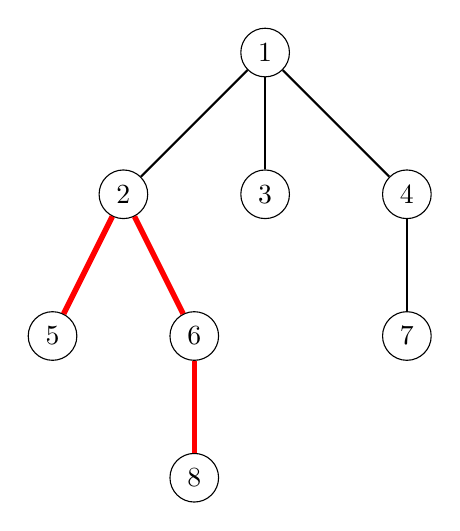
\begin{tikzpicture}[scale=0.9]
\node[draw, circle] (1) at (0,3) {$1$};
\node[draw, circle] (2) at (2,1) {$4$};
\node[draw, circle] (3) at (-2,1) {$2$};
\node[draw, circle] (4) at (0,1) {$3$};
\node[draw, circle] (5) at (2,-1) {$7$};
\node[draw, circle] (6) at (-3,-1) {$5$};
\node[draw, circle] (7) at (-1,-1) {$6$};
\node[draw, circle] (8) at (-1,-3) {$8$};
\path[draw,thick,-] (1) -- (2);
\path[draw,thick,-] (1) -- (3);
\path[draw,thick,-] (1) -- (4);
\path[draw,thick,-] (2) -- (5);
\path[draw,thick,-] (3) -- (6);
\path[draw,thick,-] (3) -- (7);
\path[draw,thick,-] (7) -- (8);

\path[draw=red,thick,-,line width=2pt] (8) -- node[font=\small] {} (7);
\path[draw=red,thick,-,line width=2pt] (7) -- node[font=\small] {} (3);
\path[draw=red,thick,-,line width=2pt] (6) -- node[font=\small] {} (3);
\end{tikzpicture}
\end{center}

Tổ tiên chung thấp nhất của các đỉnh 5 và 8 là đỉnh 2.
Các độ sâu của các đỉnh là
$\texttt{depth}(5)=3$, $\texttt{depth}(8)=4$ và $\texttt{depth}(2)=2$,
vì vậy khoảng cách giữa các đỉnh 5 và 8 là
$3+4-2\cdot2=3$.

\section{Thuật toán ngoại tuyến}

\index{offline algorithm}
\index{thuật toán ngoại tuyến}

Cho đến nay, chúng ta đã thảo luận về các thuật toán \emph{trực tuyến}
cho các truy vấn trên cây.
Các thuật toán đó có khả năng xử lý
các truy vấn lần lượt để
mỗi truy vấn được trả lời trước khi nhận truy vấn tiếp theo.

Tuy nhiên, trong nhiều bài toán, tính chất trực tuyến
là không cần thiết.
Trong phần này, chúng ta tập trung vào các thuật toán \emph{ngoại tuyến}.
Các thuật toán đó được cung cấp một tập hợp các truy vấn mà có thể
được trả lời theo bất kỳ thứ tự nào.
Thường thì dễ dàng hơn để thiết kế một thuật toán ngoại tuyến
so với một thuật toán trực tuyến.

\subsubsection{Gộp cấu trúc dữ liệu}

\index{merging data structures}
\index{gộp cấu trúc dữ liệu}

Một phương pháp để xây dựng một thuật toán ngoại tuyến
là thực hiện một duyệt cây theo chiều sâu
và duy trì các cấu trúc dữ liệu trong các đỉnh.
Tại mỗi đỉnh $s$, chúng ta tạo ra một cấu trúc dữ liệu
$\texttt{d}[s]$ dựa trên
các cấu trúc dữ liệu của các con của $s$.
Sau đó, bằng cách sử dụng cấu trúc dữ liệu này,
tất cả các truy vấn liên quan đến $s$ được xử lý.

Như một ví dụ, hãy xem xét bài toán sau:
cho một cây và một tập hợp các đường đi, nhiệm vụ của chúng ta là
tìm số lượng đường đi tối đa giao nhau tại một đỉnh.
Ví dụ, hãy xem xét cây sau và các đường đi
$1 \to 8$, $5 \to 7$ và $6 \to 9$:
\begin{center}
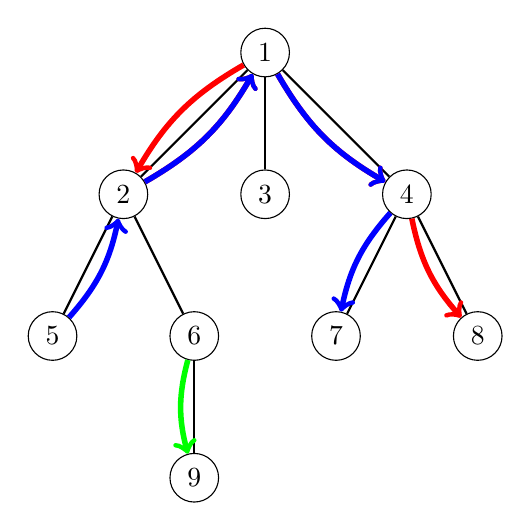
\begin{tikzpicture}[scale=0.9]
\node[draw, circle] (1) at (0,3) {$1$};
\node[draw, circle] (2) at (-2,1) {$2$};
\node[draw, circle] (3) at (0,1) {$3$};
\node[draw, circle] (4) at (2,1) {$4$};
\node[draw, circle] (5) at (-3,-1) {$5$};
\node[draw, circle] (6) at (-1,-1) {$6$};
\node[draw, circle] (7) at (1,-1) {$7$};
\node[draw, circle] (8) at (3,-1) {$8$};
\node[draw, circle] (9) at (-1,-3) {$9$};

\path[draw,thick,-] (1) -- (2);
\path[draw,thick,-] (1) -- (3);
\path[draw,thick,-] (1) -- (4);
\path[draw,thick,-] (2) -- (5);
\path[draw,thick,-] (2) -- (6);
\path[draw,thick,-] (4) -- (7);
\path[draw,thick,-] (4) -- (8);
\path[draw,thick,-] (6) -- (9);

\path[draw=red,thick,->,line width=2pt] (1) edge [bend right=15] (2);
\path[draw=red,thick,->,line width=2pt] (2) edge [bend right=15] (1);
\path[draw=red,thick,->,line width=2pt] (1) edge [bend right=15] (4);
\path[draw=red,thick,->,line width=2pt] (4) edge [bend right=15] (8);

\path[draw=blue,thick,->,line width=2pt] (5) edge [bend right=15] (2);
\path[draw=blue,thick,->,line width=2pt] (2) edge [bend right=15] (1);
\path[draw=blue,thick,->,line width=2pt] (1) edge [bend right=15] (4);
\path[draw=blue,thick,->,line width=2pt] (4) edge [bend right=15] (7);

\path[draw=green,thick,->,line width=2pt] (6) edge [bend right=15] (9);
\end{tikzpicture}
\end{center}
Trong trường hợp này, câu trả lời là 2, vì các đường đi $1 \to 8$ và $5 \to 7$
giao nhau tại các đỉnh 1, 2 và 4.

Chúng ta có thể giải quyết bài toán này bằng cách sử dụng một thuật toán ngoại tuyến.
Ý tưởng là biểu diễn mỗi đường đi từ $a$ đến $b$
bằng cách thêm $+1$ tại các đỉnh $a$ và $b$
và $-1$ tại tổ tiên chung thấp nhất của $a$ và $b$
và (nếu có) cha của nó.
Sau đó, đối với mỗi đỉnh $s$, tổng các giá trị trong cây con của nó
cho biết có bao nhiêu đường đi đi qua $s$.
Câu trả lời cho bài toán là tổng tối đa.

Ví dụ, trong cây trên,
tổ tiên chung thấp nhất của 1 và 8 là 1,
tổ tiên chung thấp nhất của 5 và 7 là 1,
và tổ tiên chung thấp nhất của 6 và 9 là 6.
Do đó, các giá trị sau được thêm vào cây:
\begin{itemize}
\item đường đi $1 \to 8$: $+1$ tại 1 và 8, $-1$ tại 1
\item đường đi $5 \to 7$: $+1$ tại 5 và 7, $-1$ tại 1
\item đường đi $6 \to 9$: $+1$ tại 6 và 9, $-1$ tại 6 và 2
\end{itemize}
Lưu ý rằng vì đỉnh 1 là gốc, nó không có cha.
Ngoài ra, chúng ta thêm hai lần $-1$ cho đường đi $6 \to 9$
vì tổ tiên chung thấp nhất (6) không phải là điểm cuối.

Các giá trị cuối cùng trong cây và các tổng cây con là như sau:
\begin{center}
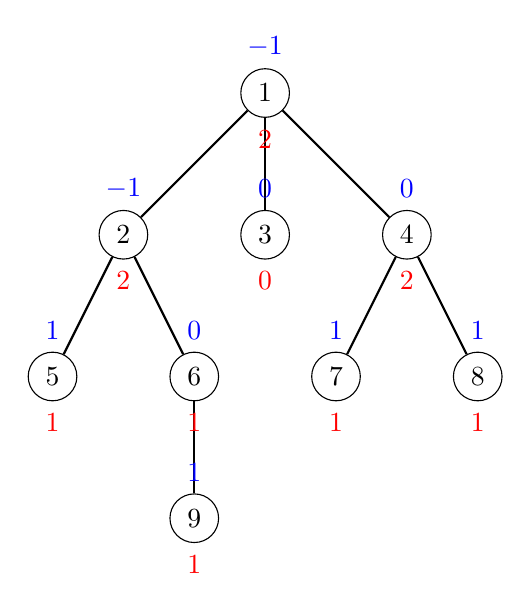
\begin{tikzpicture}[scale=0.9]
\node[draw, circle] (1) at (0,3) {$1$};
\node[draw, circle] (2) at (-2,1) {$2$};
\node[draw, circle] (3) at (0,1) {$3$};
\node[draw, circle] (4) at (2,1) {$4$};
\node[draw, circle] (5) at (-3,-1) {$5$};
\node[draw, circle] (6) at (-1,-1) {$6$};
\node[draw, circle] (7) at (1,-1) {$7$};
\node[draw, circle] (8) at (3,-1) {$8$};
\node[draw, circle] (9) at (-1,-3) {$9$};

\path[draw,thick,-] (1) -- (2);
\path[draw,thick,-] (1) -- (3);
\path[draw,thick,-] (1) -- (4);
\path[draw,thick,-] (2) -- (5);
\path[draw,thick,-] (2) -- (6);
\path[draw,thick,-] (4) -- (7);
\path[draw,thick,-] (4) -- (8);
\path[draw,thick,-] (6) -- (9);

\node[color=blue] at (0,3.65) {$-1$};
\node[color=blue] at (-2,1.65) {$-1$};
\node[color=blue] at (0,1.65) {$0$};
\node[color=blue] at (2,1.65) {$0$};
\node[color=blue] at (-3,-0.35) {$1$};
\node[color=blue] at (-1,-0.35) {$0$};
\node[color=blue] at (1,-0.35) {$1$};
\node[color=blue] at (3,-0.35) {$1$};
\node[color=blue] at (-1,-2.35) {$1$};

\node[color=red] at (0,2.35) {$2$};
\node[color=red] at (-2,0.35) {$2$};
\node[color=red] at (0,0.35) {$0$};
\node[color=red] at (2,0.35) {$2$};
\node[color=red] at (-3,-1.65) {$1$};
\node[color=red] at (-1,-1.65) {$1$};
\node[color=red] at (1,-1.65) {$1$};
\node[color=red] at (3,-1.65) {$1$};
\node[color=red] at (-1,-3.65) {$1$};
\end{tikzpicture}
\end{center}
Các tổng cây con tối đa là 2, đó là câu trả lời.
